%%%%%%%%%%%%%%%%%%%%%%%%%%%%%%%%%%%%%%%%%%%%%%%%%%%%%%%%%%%%%%%%%%%%%%%%%%%%%%%%
%% Title (en): Multiagent Systems and Organizations                           %%
%% Title (cs): Multiagentní systémy a organizace                              %%
%%                                                                            %%
%% Author: Bc. Lukáš Kúdela                                                   %%
%% Supervisor: Prof. RNDr. Petr Štěpánek, DrSc.                               %%
%%                                                                            %%
%% Academic year: 2011/2012                                                   %%
%%%%%%%%%%%%%%%%%%%%%%%%%%%%%%%%%%%%%%%%%%%%%%%%%%%%%%%%%%%%%%%%%%%%%%%%%%%%%%%%

\chapter{Examples}

% Chapter - intro
In this chapter, we will present examples demonstrating the usage of the Thespian4Jade library (ALT: module), an extension of the Jade framework.
The examples are ordered by the complexity of the MAS social structure; the first can be considered a toy problem, while the last one is toy problem by no means.

% Examples - structure - specification & manifestation
The MAS in each example is presented in two parts: specification and manifestation.
The specification part presents the model of the MAS and the manifestation part presents a run of the MAS.

%%%%%%%%%%%%%%%%%%%%%%%%%%%%%%%%%%%%%%%%%%%%%%%%%%%%%%%%%%%%%%%%%%%%%%%%%%%%%%%%
\section{Example 1: Function Invocations}
%%%%%%%%%%%%%%%%%%%%%%%%%%%%%%%%%%%%%%%%%%%%%%%%%%%%%%%%%%%%%%%%%%%%%%%%%%%%%%%%

%%%%%%%%%%%%%%%%%%%%%%%%%%%%%%%%%%%%%%%%%%%%%%%%%%%%%%%%%%%%%%%%%%%%%%%%%%%%%%%%
\subsection*{MAS Specification}

\subsubsection*{Organization Part}

% Function invocation organization
This example demonstrates a simple organization - the \textit{Invoke function} organization (modelled by the \texttt{FunctionInvocation\_Organization} agent class).
% Function invocation organization - purpose
The purpose of the organization is to facilitate function invocation by grouping two agents: the first agent \textit{invokes} a function and the second agent \textit{executes} it.
Thus, the function is invoked in a \textit{remote} way.
The example uses the factorial function, but it should be obvious that any (computable) function can be used instead.

% Function invocation organization - roles
The \textit{Invoke function} organization contains two roles - \textit{Asker} and \textit{Answerer} - and one protocol - \textit{Invoke function}.

% Invoker role
The \textit{Invoker} role (modelled by the \texttt{Invoker\_Role} class) is a single role representing an invoker of a function.
The invoker of a function can request the executer to compute the function.
% Invoker role - competences & responsibilities
The \textit{Invoker} role has one competence - \textit{Invoke function} - and no responsibilities.

% Invoke function competence
The \textit{Invoke function} competence (modelled by the \texttt{InvokeFunction\_Competence} class) is a competence to invoke a function.
% Invoke function competence - argument & result
The competence has one argument - the function argument - and one result - the function value.

% Executer role
The \textit{Executer} role (modelled by the \texttt{Executer\_Role} class) is a single role representing an executer of a function.
The executer function can compute the function upon request.
% Execute role - competences & responsibilities
The \textit{Executer} role has no competences and one responsibility - \textit{Execute function}.

% Execute function responsibility
The \textit{Execute function} responsibility (modelled by the \texttt{ExecuteFunction\_Responsibility} class) is a responsibility to execute a function together with its argument.
% Execute function responsibility - argument & result
The responsibility has one argument - the function argument - and one result - the function value.

\subsubsection*{Protocol Part}

% Invoke function protocol
The \textit{Invoke function} protocol (modelled by the \texttt{InvokeFunctionProtocol}) is a protocol by which the initiator party (modelled by the \texttt{InvokeFunction\_InitiatorParty} class) requests the responder party (modelled by the \texttt{InvokeFunction\_ResponderParty}) to execute a function (the factorial function in this example).

% Request message
The \textit{Request} message (modelled by the \texttt{RequestMessage} class) is a message sent by the \textit{Invoker} to the \textit{Executer} carrying a request to execute the function and its argument.

% Reply message
The \textit{Reply} message (modelled by the \texttt{ReplyMessage} class) is a message sent by the \textit{Executer} to the \textit{Invoker} carrying an information that the function has been executed and its value.

\subsubsection*{Player Part}

% Demo player
The \textit{Demo} player (modelled by the \texttt{Demo\_Player} agent class) is a player capable of computing (ALT: evaluating) the factorial function.

%%%%%%%%%%%%%%%%%%%%%%%%%%%%%%%%%%%%%%%%%%%%%%%%%%%%%%%%%%%%%%%%%%%%%%%%%%%%%%%%
\subsection*{Manifestation}

% Agents - players & organizations
There are two \textit{Demo} players in the running MAS: \textit{demo1} (modelled by the \texttt{demo1\_Player} agent instance) plays the role of \textit{Invoker} and \textit{demo2} (modelled by the \texttt{demo2\_Player} agent instance) plays the role of \textit{Executer} in the \textit{invoke function} organization (modelled by the \texttt{invokeFunction\_Organization} agent instance).

\subsubsection*{Stage 1 - Role Enactment}

% Figure: Stage 1 - Role enactment
\begin{figure}[H]
	\centering
	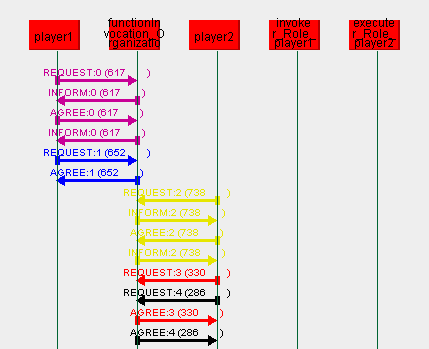
\includegraphics[width=\textwidth]{images/example1-stage1.png}
	\caption{Stage 1 - Role enactment}
	\label{figure:example1-stage1}
\end{figure}

\subsubsection*{Stage 2: Role Activation}

% Figure: Stage 2 - Role activation
\begin{figure}[H]
	\centering
	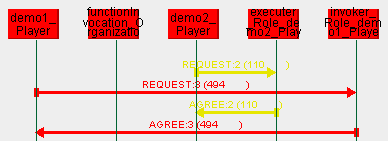
\includegraphics[width=\textwidth]{images/example1-stage2.png}
	\caption{Stage 2 - Role activation}
	\label{figure:example1-stage2}
\end{figure}

\subsubsection*{Stage 3: Competence and Responsibility Invocation}

% Figure: Stage 3 - Competence and responsibility invocation
\begin{figure}[H]
	\centering
	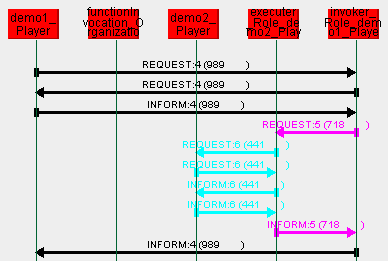
\includegraphics[width=\textwidth]{images/example1-stage3.png}
	\caption{Stage 3 - Competence and responsibility invocation}
	\label{figure:example1-stage3}
\end{figure}

\subsubsection*{Stage 4: Role Deactivation}

% Figure: Stage 4 - Role deactivation
\begin{figure}[H]
	\centering
	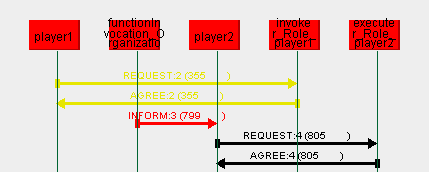
\includegraphics[width=\textwidth]{images/example1-stage4.png}
	\caption{Stage 4 - Role deactivation}
	\label{figure:example1-stage4}
\end{figure}

\subsubsection*{Stage 5: Role Deactment}

% Figure: Stage 5 - Role deactment
\begin{figure}[H]
	\centering
	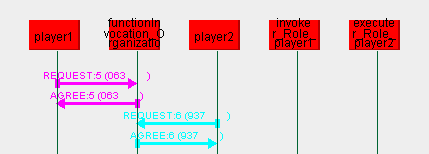
\includegraphics[width=\textwidth]{images/example1-stage5.png}
	\caption{Stage 5 - Role deactment}
	\label{figure:example1-stage5}
\end{figure} 

%%%%%%%%%%%%%%%%%%%%%%%%%%%%%%%%%%%%%%%%%%%%%%%%%%%%%%%%%%%%%%%%%%%%%%%%%%%%%%%%
\section{Example 2: Expression Evaluation}
%%%%%%%%%%%%%%%%%%%%%%%%%%%%%%%%%%%%%%%%%%%%%%%%%%%%%%%%%%%%%%%%%%%%%%%%%%%%%%%%

%%%%%%%%%%%%%%%%%%%%%%%%%%%%%%%%%%%%%%%%%%%%%%%%%%%%%%%%%%%%%%%%%%%%%%%%%%%%%%%%
\subsection*{Specification}

\subsubsection*{Organization Part}

\subsubsection*{Protocol Part}

\subsubsection*{Player Part}

%%%%%%%%%%%%%%%%%%%%%%%%%%%%%%%%%%%%%%%%%%%%%%%%%%%%%%%%%%%%%%%%%%%%%%%%%%%%%%%%
\subsection*{Manifestation}

%%%%%%%%%%%%%%%%%%%%%%%%%%%%%%%%%%%%%%%%%%%%%%%%%%%%%%%%%%%%%%%%%%%%%%%%%%%%%%%%
\section{Example 3: Auction}
%%%%%%%%%%%%%%%%%%%%%%%%%%%%%%%%%%%%%%%%%%%%%%%%%%%%%%%%%%%%%%%%%%%%%%%%%%%%%%%%

%%%%%%%%%%%%%%%%%%%%%%%%%%%%%%%%%%%%%%%%%%%%%%%%%%%%%%%%%%%%%%%%%%%%%%%%%%%%%%%%
\subsection*{Specification}

\subsubsection*{Organization Part}

% Auction organization
This example demonstrates a relatively complex organization - the \textit{Auction} organization (modelled by the \texttt{Auction\_Organization} agent class).
% Auction organization - purpose
The purpose of the organization is to facilitate an auction by grouping three or more agents: one agent \textit{auctions} an item and the other agents \textit{bid} for it.
The item can be auctioned in an envelope, Vickrey, english or dutch auction.
The example uses the envelope auction to sell works of art, but it should be apparent that any of the four auction types can be used to sell any items.

% Auction organization - roles
The \textit{Auciton} organization has two roles - \textit{Auctioneer} and \textit{Bidder} - and four protocols - \textit{Envelope auction}, \textit{Vickrey auction}, \textit{English auction} and \textit{Dutch auction}.

% Auctioneer role
The \textit{Auctioneer} role (modelled by the \texttt{Auctioneer\_Role} class) is a single role representing an auctioneer in an auction.
The auctioneer is an auction participant trying to sell the auctioned item.
There is only one auctioneer, hence the single role.
% Auctioneer role - competences & responsibilities
The \textit{Auctioneer} has one competence - \textit{Auction} - and no responsibilities.

% Auction competence
The \textit{Auction} competence (modelled by the \texttt{Auction\_Competence} class) is a competence to auction an item.
% Auction competence - argument & result
The competence has several arguments - TODO - and several results - TODO.

% Bidder role
The \textit{Bidder} role (modelled by the \texttt{Bidder\_Role} class) is a multiple role representing a bidder in an auction.
A bidder is an auction participant attempting to buy the auctioned item.
There are many bidders, hence the multiple role.
% Bidder role - competences & responsibilities
It has no competences and one responsibility - \textit{Bid}.

% Bidder responsibility
The \textit{Bid} responsibility (modelled by the \texttt{Bid\_Responsibility} class) is a responsibility to bid for an item.
% Bidder responsibility - argument & result
The responsibility has several arguments - TODO - and several results - TODO.

\subsubsection*{Protocol Part}

% Envelope acution protocol
The \textit{Envelope auction} protocol (modelled by the \texttt{EnvelopeAuctionProtocol} class) is a protocol defining the Envelope auction.
The Envelope auction is ... TODO.

% Vickrey auction protocol
The \textit{Vickrey auction} protocol (modelled by the \texttt{VickreyAuctionProtocol} class) is a protocol defining the Vickrey auction.
The Vickrey auction is ... TODO.

% English auction protocol
The \textit{English auction} protocol (modelled by the \texttt{EnglishAuctionProtocol} class) is a protocol defining the English auction. 
The English auction is ... TODO.

% Dutch auction protocol
The \textit{Dutch auction} protocol (modelled by the \texttt{DutchAuctionProtocol} class) is a protocol defining the Dutch auction.
The Dutch auction is ... TODO.

% AuctionCFP message
The \textit{Auction CFP} message (modelled by the \texttt{AuctionCFPMessage}) is a message sent by the \textit{Auctioneer} to all \textit{Bidders} carrying an auction call-for-proposal together with the auctioned item's name.

% Bid message
The \textit{bid} message (modelled by the \texttt{BidMessage}) is a message sent by a \textit{Bidder} to the \textit{Auctioneer} carrying information that a bid has been made together with the bid.

\subsubsection*{Player Part}

% Participant player
The \textit{Participant} player (modelled by the \texttt{Participant\_Player} agent class) is a player capable of bidding in an auction.

%%%%%%%%%%%%%%%%%%%%%%%%%%%%%%%%%%%%%%%%%%%%%%%%%%%%%%%%%%%%%%%%%%%%%%%%%%%%%%%%
\section{Manifestation}

% Agents - players & organizations
There are three players of this type in the running MAS: \textit{participant1} (modelled by the \texttt{participant1\_Player} agent instance), \textit{participant2} (modelled by the \texttt{participant2\_Player} agent instance) and \textit{participant3} (modelled by the \texttt{participant3\_Player} agent instance) taking turns in playing the \textit{Auctioneer} role and \textit{Bidder} roles in the \textit{auction} organization (modelled by the \textit{auction\_Organization} agent instance).

\subsubsection*{Stage 1 - Role Enactment}

% Figure: Stage 1 - Role enactment
\begin{figure}[H]
	\centering
	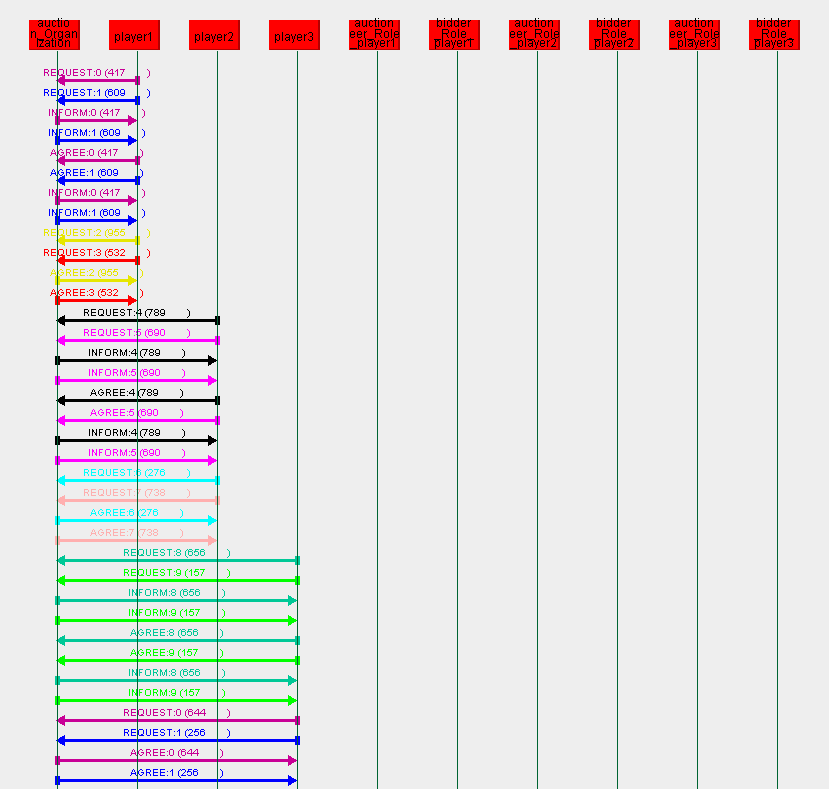
\includegraphics[width=\textwidth]{images/example3-stage1.png}
	\caption{Stage 1 - Role enactment}
	\label{figure:example3-stage1}
\end{figure}

\subsubsection*{Stage 2: Role Activation}

% Figure: Stage 2 - Role activation
\begin{figure}[H]
	\centering
	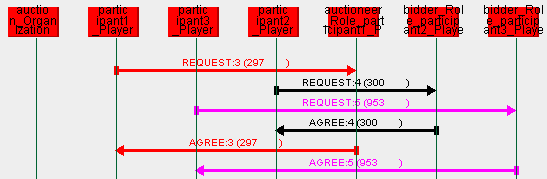
\includegraphics[width=\textwidth]{images/example3-stage2.png}
	\caption{Stage 2 - Role activation}
	\label{figure:example3-stage2}
\end{figure}

\subsubsection*{Stage 3: Competence and Responsibility Invocation}

% Figure: Stage 3 - Competence and responsibility invocation
\begin{figure}[H]
	\centering
	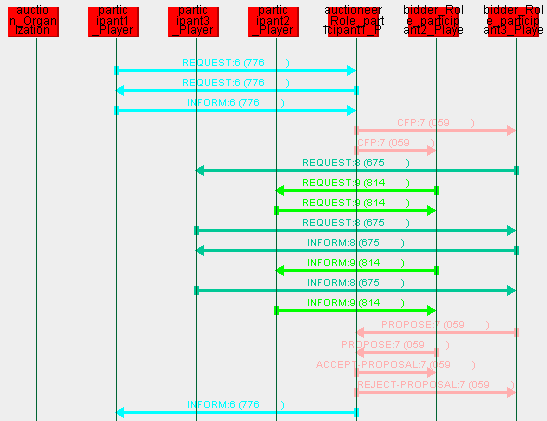
\includegraphics[width=\textwidth]{images/example3-stage3.png}
	\caption{Stage 3 - Competence and responsibility invocation}
	\label{figure:example3-stage3}
\end{figure}

\subsubsection*{Stage 4: Role Deactivation}

% Figure: Stage 4 - Role deactivation
\begin{figure}[H]
	\centering
	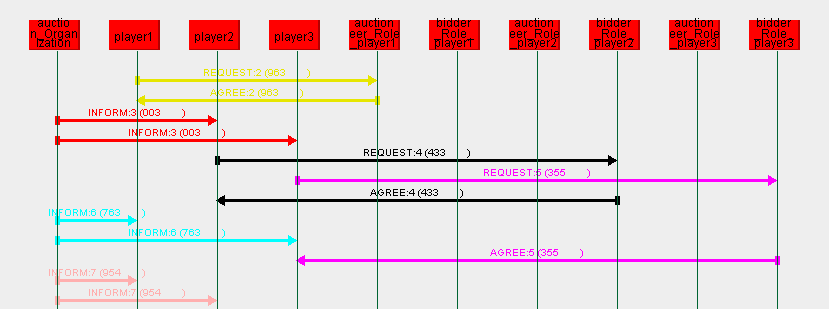
\includegraphics[width=\textwidth]{images/example3-stage4.png}
	\caption{Stage 4 - Role deactivation}
	\label{figure:example3-stage4}
\end{figure}

\subsubsection*{Stage 5: Role Deactment}

% Figure: Stage 5 - Role deactment
\begin{figure}[H]
	\centering
	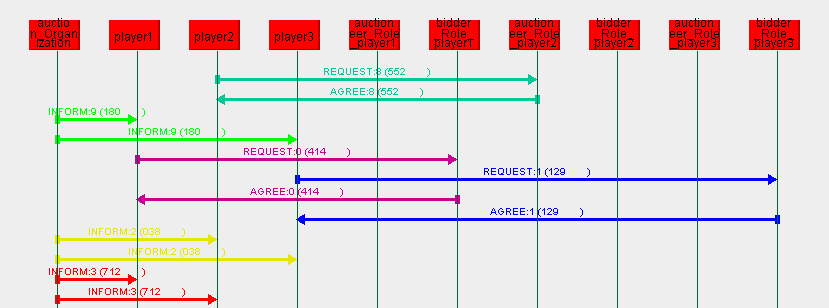
\includegraphics[width=\textwidth]{images/example3-stage5.png}
	\caption{Stage 5 - Role deactment}
	\label{figure:example3-stage5}
\end{figure} 